
\subsection{\textit{One more thing}}

\subsubsection{\texttt{dynamic}}

Afin de saisir relativement rapidement les séances correspondantes à un semestre
complet, nous avons utilisé des prédicats travaillant sur des listes.
L'inconvénient est la charge de travail supplémentaire demandé à Prolog à chaque
prédicat \texttt{seance/4}, par exemple.
Toutes ces données étant disponible à priori, nous avons donc utilisé le
prédicat Prolog \texttt{dynamic} qui permet de définir des prédicats à la volée,
comme un chargement de base de données.

Cette transformation a permit un gain d'un facteur 100, passant de 10min à 6s
pour la planification du même jeu de données.

\subsubsection{Optimisation de l'emploi du temps}

Afin de rendre l'emploi du temps un peu plus vivable, on peut optimiser un peu
les choses.

Évitons de planifier des cours en début ou fin de journée :

\begin{lstlisting}[language=Prolog, caption=Éviter début et fin de journée,
captionpos=b, label={lst:debutfin}]
% plage(H, _, _).
member(H, [2, 3, 4, 5, 1, 6]), % une plage horaire
                               % evitons premier et dernier creneau
\end{lstlisting}

Limitons le nombre de cours par jours :

\begin{lstlisting}[language=Prolog, caption=Limite de cours par jour,
captionpos=b, label={lst:nbcours}]
/**
 * tropDeCoursCeJour(+J, +M, +Max, +Cs)
 *
 * @arg J   Jour
 * @arg M   Mois
 * @arg Max Nombre max de cours par jour
 * @arg Cs  Liste de creneaux deja planifies
 */
tropDeCoursCeJour(J, M, Max, Cs) :-
    findall(S, member([S, _, J, M, _], Cs), Csjour),
    length(Csjour, X),
    X > Max.
\end{lstlisting}

Empêchons les cours le jeudi après-midi :

\begin{lstlisting}[language=Prolog, caption=Jeudi après-midi,
captionpos=b, label={lst:jeudi}]
/**
 * jeudiApresMidi(+H, +J)
 *
 * Est vrai si le moment passe est un jeudi apres midi
 *
 * Partant du principe qu'il y a 5 jours dans une semaine et que l'annee
 * commence un lundi, sans cas particulier, alors les jeudis tombent le 4eme
 * jour de chaque semaine.
 *
 * @arg H   Plage horaire
 * @arg J   Jour
 */
jeudiApresMidi(H, J) :-
    (J + 1) mod 5 is 0,
    H > 3.
\end{lstlisting}

Limitons à un examen par jour :

\begin{lstlisting}[language=Prolog, caption=Détection de conflit d'exament,
captionpos=b, label={lst:examen}]
/**
 * conflitExamen(+S, +J, +M, +C)
 *
 * Est vrai si C se deroule le meme jour et que les deux creneaux sont des
 * examents
 *
 * @arg S   Seance
 * @arg J   Jour
 * @arg M   Mois
 * @arg C   Un creneau
 */
conflitExamen(S, J, M, [S2, _, J, M, _]) :-
    seance(S, ds, _, _),
    seance(S2, ds, _, _).
\end{lstlisting}

L'intégration de ces prédicats est disponible dans le code joint au rendu.

\subsubsection{Affichage}
\begin{lstlisting}[language=Prolog, caption=Affichage, captionpos=b,
label={lst:affi}]
/**
 * afficherPlanification(+Cs)
 *
 * Affiche la planification dans l'ordre chronologique
 *
 * @arg Cs  Une liste de creneaux
 */
afficherPlanification([]) :- !.
afficherPlanification(Cs) :-
    date(J, M),
    plage(H, _, _),
    member(C, Cs),
    C = [S, H, J, M, L],
    write('--------------------------------------------------------------'), nl,
    afficherSeance(S), nl,
    afficherMoment(J, M, H), nl,
    afficherGroupes(S), nl,
    afficherProfs(S), nl,
    afficherSalle(L), nl,
    delete(Cs, C, Cs2),
    afficherPlanification(Cs2),
    !.
\end{lstlisting}

Pour l'affichage, on utilise la fonction \texttt{afficherPlanification(+Cs)} que l'on peut voir dans l'algorithme \ref{lst:affi} ci-dessus.

On va chercher à afficher l'emploi du temps par ordre chronologie : donc du premier jour, première plage jusqu'au dernier jour, dernière plage.

De ce fait, la fonction récupère tout d'abord, la date. Puis dans un second temps une plage.

Ensuite, elle sélectionne un des créneaux qui correspond et débute l'affichage.

\begin{lstlisting}[language=Prolog, caption=Affichage, captionpos=b,
label={lst:affi_sea}]
/**
 * afficherSeance(+S)
 *
 * @arg S
 */
afficherSeance(S) :-
    seance(S, TypeCours, Mat, Nom),
    write('Seance:\t\t'),
    write(S), write(' "'), write(Nom), write('"'),
    write(' - '), write(TypeCours),
    write(' - '), write(Mat).
\end{lstlisting}

Celui-ci est atomique, on affiche tout d'abord la séance (Nom, type, matière), puis le moment (Jour, mois et plage) ainsi de suite jusqu'à avoir toutes les informations propres à un emploi du temps pour ce créneau.
Sur l'algorithme \ref{lst:affi_sea} ci-dessus, on a un exemple de fonction : celle permettant d'afficher les séances.

On supprime ensuite ce créneau de la liste des créneaux vu qu'il a déjà été affiché puis on rappelle la fonction sur la nouvelle liste.

On peut voir le rendu de l'affichage sur l'image \ref{fig:affi_sortie}.

\begin{figure}[t]
	\centering
    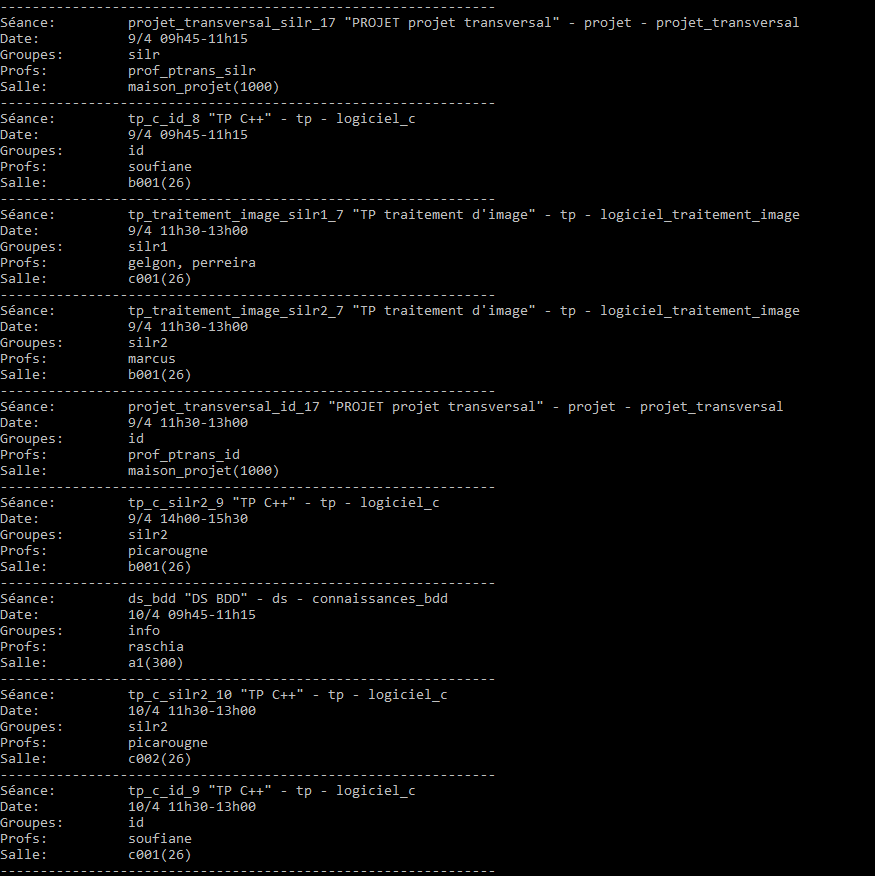
\includegraphics[keepaspectratio=true,width=12cm]{affichage.png}
        \caption{\label{fig:affi_sortie} Affichage en console}
\end{figure}


\subsubsection{Tests}

Les prédicats sont testés à l'aide PLUnit sur notre premier jeu de données
\texttt{instance\_old.pl}. Avoir une démarche TDD (Test Driven Development) nous
a grandement aidé à la découpe du problème. Cela nous a également permit
d'arriver rapidement à un code de qualité et de pouvoir travailler à
l'amélioration et aux performances de notre solution.

Voici un exemple :

\begin{lstlisting}[language=Prolog, caption=Exemple de test, captionpos=b,
label={lst:test}]
:- begin_tests(indiceSeance).

test("indiceSeance renvoie 0 si la seance ne suit rien") :-
    indiceSeance(1, 0).

test("indiceSeance renvoie le nombre de seances precedentes sinon") :-
    indiceSeance(2, 1),
    indiceSeance(8, 2).

:- end_tests(indiceSeance).
\end{lstlisting}

\begin{lstlisting}[language=bash, caption=Lancer les tests, captionpos=b]
swipl -s run_tests.pl
\end{lstlisting}


\subsubsection{Question subsidiaire}

L'algorithme \texttt{planifier(+Ss, +Ds, -Cs)} permet également de planifier des
séances dans un emploi du temps déjà réalisé (\texttt{Ds}).

\begin{lstlisting}[language=Prolog, caption=Exemple d'ajout dans un EDT, captionpos=b,
label={lst:creneauValideCreneau}]
findall(S, seance(S, _, _, _), Ss), % toutes les seances
predsort(beforeSeance, Ss, Ss2),
reverse(Ss2, [X|Ss3]), % X est une seance qu'on ne veut pas planifier tout
                       % de suite
planifier(Ss3, Cs), % premier emploi du temps

planifier([X], Cs, Cs2). % ajout de X sur dans l'emploi du temps si possible
\end{lstlisting}

